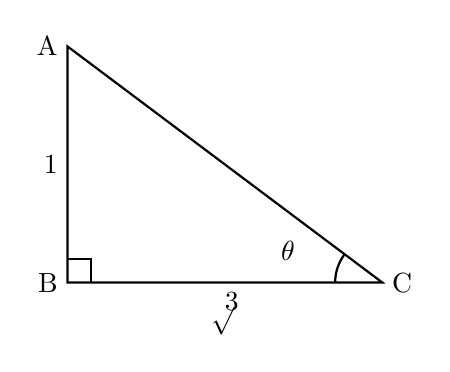
\begin{tikzpicture}[scale=1]

    % Define the vertices of the right-angled triangle
    \coordinate (B) at (0,0);
    \coordinate (C) at (4,0);
    \coordinate (A) at (0,3);

    % Draw the triangle
    \draw[thick] (A) -- (B) -- (C) -- cycle;

    % Draw the right-angle symbol at B
    \draw[thick] (B) ++(0.3,0) -- ++(0,0.3) -- ++(-0.3,0);

    % Draw the angle arc at C for theta
    \draw[thick] (C) ++(180:0.6) arc (180:143.1:0.6);

    % Add labels for the vertices
    \node[left] at (A) {A};
    \node[left] at (B) {B};
    \node[right] at (C) {C};

    % Add length labels for the sides
    % Length 1 for the height AB
    \node[left] at (0,1.5) {1};
    % Length \sqrt{3} for the base BC
    \node[below] at (2,0) {\raisebox{-6.5pt}{$\surd$}$\!\!3$};

    % Add the angle label theta
    \node at (2.8, 0.4) {$\theta$};

\end{tikzpicture}